\chapter{Evaluation}
\label{ch:Evaluation}

In this chapter the prototype is evaluated in terms of its functionality and its properties.

All possible valid configurations will be generate for one use case i.e. all possible valid configurations for the forest use case.

Generate groups with preferences (explicit preferences) and configuration state (which would be for example the currently existing forest).

\section{Metric}
\label{sec:Evaluation:Metrics}

For the evaluation a metric to evaluate by is needed. The proposed metric for usage is that of satisfactions. Satisfaction is quantified in this thesis by a threshold metric. A user's preference is used to calculate a rating for each possible solution. The score will be calculated using the average of a user's rating for each characteristic that is part of the solution. The result allows that a configuration can be compared to all other configurations and ranked according to the percentage of configurations that it beats. The threshold metric consists of two parameters. First the threshold center $tc$ and second the satisfaction distance $sd$. The threshold for a person being satisfied is $tc + sd$ and of a person being dissatisfied at $tc - sd$. If a recommendation lies in between these two thresholds the person is classified to neither by satisfied nor be unsatisfied with the solution. For this thesis  $sd=5\%$ will be used. This choice is guided by the assumption that people switch from satisfied to unsatisfied rather quickly. Therefore the parameter considered in this thesis is the $tc$. An example is the choice of $tc = 60\%$. This results in a person being satisfied if recommendation is better than at lest $65\%$ of possible finished configurations. Moreover, a person is dissatisfied if the recommendation is only better than $55\%$ of possible finished configurations. A recommendation that is better than at least $55\%$ and not better than $65\%$ of possible solutions is considered neutral by the individual.
Different $tc$ values allow to model different situations. A situation where there is a low willingness to compromise is modelled by a high $tc$. A contrary situation where a group has a high willingness to compromise is modelled by a low $tc$.

\section{Questions to Answer During the Evaluation}
\label{sec:Evaluation:Questions}

\begin{itemize}
    \item Main question: How does the satisfaction with a group decision, guided by a the recommender, differ from the decision of a single decision maker, who does not take the other group member's opinion into account?
    \item How many group members are satisfied with the group decision on average?
    %\item Is the recommender fair, i.e. no user type is always worse off than others? (Just uses groupe preferences)
    \item How does the amount of stored finished configurations relate to recommendation satisfaction?
\end{itemize}

\section{Effect of Stored Finished Configurations}
\label{sec:Evaluation:EffectFinishedConfiguration}

When evaluating just a subset of stored finished configurations it is important to avoid outliers. This is the reason why a process inspired by cross validation is used. The configuration database is randomly ordered and sliced into sub databases of the needed size. As an example, if the evaluated stored data size is 20, a configuration database containing 100 configurations is split into five sub databases of size 20. Now the evaluation is done on each of the sub databases and as a result the average is taken.

\section{Use Case}
\label{sec:Evaluation:UseCase}

To evaluate data a given use case is needed. In this thesis a forestry use case is evaluated. This is a use case with four stakeholders. \autoref{fig:Concept:ForestExample} already presented the attributes and characteristics used in this use case but an extension is needed to fully show the whole use case. Namely rules of non valid configurations. The constraints for this use case are listed in not with form in \autoref{tab:Evaluation:UseCase}. 

\begin{table}
    \begin{center}
        \begin{tabular}{r|l}
            & not with (either of the listed) \\
            \hline
            $(\textit{indigenous}, \text{moderate})$   & $(\textit{resilient}, \text{high})$ \\
            \hline
            $(\textit{indigenous}, \text{high})$   & $(\textit{resilient}, \text{high}), (\textit{usable}, \text{moderate}), (\textit{usable}, \text{high}),$ \\
            & $(\textit{quantity}, \text{high}), (\textit{price}, \text{low})$ \\
            \hline 
            $(\textit{resilient}, \text{moderate})$   & $(\textit{usable}, \text{high})$ \\
            \hline
            $(\textit{resilient}, \text{high})$   & $(\textit{usable}, \text{high}), (\textit{usable}, \text{moderate}), (\textit{quantity}, \text{high}),$ \\
            & $(\textit{price}, \text{moderate}), (\textit{price}, \text{low})$ \\
            \hline
            $(\textit{usable}, \text{low})$ & $(\textit{quantity}, \text{high}), (\textit{price}, \text{moderate}), (\textit{price}, \text{low})$\\
            \hline
            $(\textit{usable}, \text{high})$ & $(\textit{accessibility}, \text{high})$\\
            \hline
            $(\textit{effort}, \text{manual})$ & $(\textit{quantity}, \text{high}), (\textit{price}, \text{low}), (\textit{price}, \text{moderate})$\\
            \hline
            $(\textit{effort}, \text{harvester})$ & $(\textit{accessibility}, \text{high}), (\textit{accessibility}, \text{moderate})$\\
            \hline
            $(\textit{effort}, \text{autonomous})$ & $(\textit{accessibility}, \text{high}), (\textit{accessibility}, \text{moderate})$\\
            \hline
            $(\textit{quantity}, \text{low})$ & $(\textit{price}, \text{low}), (\textit{price}, \text{moderate})$\\
            \hline
            $(\textit{quantity}, \text{moderate})$ & $(\textit{price}, \text{low}), (\textit{price}, \text{moderate})$\\
            \hline
            $(\textit{quantity}, \text{high})$ & $(\textit{accessibility}, \text{high}), (\textit{accessibility}, \text{moderate})$\\
            \hline
        \end{tabular}
        \caption{Constrains in not with form for the forest use case.}
        \label{tab:Evaluation:UseCase}
    \end{center}
\end{table}

The stakeholders of this use case are: a forest owner, an athlete, an environmentalist and a consumer. The owner sees the forest as an investment, he is interested in a high long term profit. On the other hand the consumer is interested in reasonable wood price as she uses wood for furniture and also for her fireplace. In contrast, the environmentalist is interested in a healthy forest that is not impacted negatively by human activity. Last is the athlete who is interested in good accessibility of the forest and that there is some life.  

\section{Generating Data}
\label{sec:Evaluation:GeneratingGroups}

The whole process explained in this section is visualized in \autoref{fig:Evaluation:GeneratingDataProcess}.

\begin{figure}
    \centering
    \includegraphics[width=1\textwidth]{./figures/60_evaluation/bpmn_evaluation_input_data_generation.pdf}
    \caption{The process used for generating data for the evaluation.}
    \label{fig:Evaluation:GeneratingDataProcess}
\end{figure}

\subsection{Generating Unfinished Configurations}

Unfinished configurations are generated using all finished configurations and taking a subset of the contained characteristics. This way all generated configurations will be valid and lead to valid solutions. For the results that are presented in this chapter around $\frac{1}{7} \approx 15\%$ of characteristics is kept.

\todo[inline]{why this paramter, elalobrate on that}

\subsection{Generating Preferences}

For the forest use case, the idea is that there are multiple types of user profiles. Each group profile is represented by a neutral, negative or positive attitude to an attribute value. Now during data generation the attitude is converted to a preference using a normal distribution. \autoref{fig:Evaluation:DataGeneration} shows how the user profile can be converted to preferences.

\pgfplotsset{height=5cm,width=\textwidth,compat=1.8}
\pgfmathdeclarefunction{gauss}{2}{%
  \pgfmathparse{1/(#2*sqrt(2*pi))*exp(-((x-#1)^2)/(2*#2^2))}%
}
\begin{figure}
    \begin{tikzpicture}
        \begin{axis}[
            every axis plot post/.append style={
                mark=none, domain=0:1, samples=50, smooth
            },
            axis x line*=bottom,
            xmin=0,
            xmax=1,
            ymin=0.1,
            xticklabel style={
                /pgf/number format/precision=3,
            },
            xtick={0,0.25, 0.5, 0.75,1},
            hide y axis]
          \addplot [draw=black, style={dashdotdotted}][very thick] {gauss(0.25,0.1)} node[text=black][above,pos=0.5] {negative};
          \addplot [draw=black, style={solid}][very thick] {gauss(0.5,0.05)} node[text=black][above,pos=0.48] {neutral};
          \addplot [draw=black, style={dotted}][very thick] {gauss(0.75,0.1)} node[text=black][above,pos=0.5] {positive};
        \end{axis}
        \end{tikzpicture}
 \caption{Distribution of preferences for a user type.}
\label{fig:Evaluation:DataGeneration}
\end{figure}

These user profiles can be used to generate rather homogenous groups but also to create groups that have interests that are more conflicting. The following group types are generated:

\begin{itemize}
    \item random groups (preferences are uniformly random)
    \item heterogeneous groups (people adhere to one preference profile like forest owner, athlete, consumer, environmentalist)
    \item homogeneous groups (only one preference profile for all group members which in this evaluation is the forest owner)
\end{itemize}

\text

\begin{table}
    \begin{center}
        \begin{tabular}{l|c|c|c|c}
                                                        & athlete           & forest owner      & environmentalist  & consumer          \\
            \hline
            $(\textit{indigenous}, \text{low})$         & \textbf{negative} & \textit{positive} & \textbf{negative} & neutral           \\
            $(\textit{indigenous}, \text{moderate})$    & \textit{positive} & neutral           & \textbf{negative} & neutral           \\
            $(\textit{indigenous}, \text{high})$        & \textit{positive} & \textbf{negative} & \textit{positive} & \textbf{negative} \\
            \hline
            $(\textit{resilient}, \text{low})$          & neutral           & \textit{positive} & neutral           & neutral           \\
            $(\textit{resilient}, \text{moderate})$     & \textit{positive} & neutral           & neutral           & neutral           \\
            $(\textit{resilient}, \text{high})$         & \textit{positive} & \textbf{negative} & \textbf{negative} & \textbf{negative} \\
            \hline
            $(\textit{usable}, \text{low})$             & neutral           & neutral           & neutral           & \textbf{negative} \\
            $(\textit{usable}, \text{moderate})$        & neutral           & neutral           & \textbf{negative} & neutral           \\
            $(\textit{usable}, \text{high})$            & \textbf{negative} & \textit{positive} & \textbf{negative} & \textit{positive} \\
            \hline
            $(\textit{effort}, \text{manual})$          & \textbf{negative} & neutral           & \textit{positive} & \textbf{negative} \\
            $(\textit{effort}, \text{harvester})$       & \textbf{negative} & \textit{positive} & \textbf{negative} & neutral           \\
            $(\textit{effort}, \text{autonomous})$      & \textbf{negative} & \textit{positive} & \textbf{negative} & neutral           \\
            \hline
            $(\textit{quantity}, \text{low})$           & \textit{positive} & \textbf{negative} & \textit{positive} & \textbf{negative} \\
            $(\textit{quantity}, \text{moderate})$      & neutral           & \textit{positive} & neutral           & \textbf{negative} \\
            $(\textit{quantity}, \text{high})$          & \textbf{negative} & \textit{positive} & \textbf{negative} & \textit{positive} \\
            \hline
            $(\textit{price}, \text{low})$              & neutral           & neutral           & neutral           & \textit{positive} \\
            $(\textit{price}, \text{moderate})$         & neutral           & \textit{positive} & neutral           & neutral           \\
            $(\textit{price}, \text{high})$             & neutral           & \textit{positive} & neutral           & \textbf{negative} \\
            \hline
            $(\textit{accessibility}, \text{low})$      & \textbf{negative} & \textit{positive} & \textit{positive} & neutral           \\
            $(\textit{accessibility}, \text{moderate})$ & neutral           & neutral           & neutral           & neutral           \\
            $(\textit{accessibility}, \text{high})$     & \textit{positive} & \textbf{negative} & \textbf{negative} & neutral           \\
            \hline
        \end{tabular}
        \caption{ The attitudes of each group member profile. }
        \label{tab:Evaluation:GroupMemberMappings}
    \end{center}
\end{table}



\todo[inline]{explain preference profiles}

\section{Hypotheses}
\label{sec:Evaluation:Hypotheses}

Understanding data is made easier by first posing hypothesises. This section gives an overview over the hypothesis used during data analysis.

\begin{enumerate}[font={\bfseries},label={H\arabic*}]
    \item More homogeneous groups have more satisfied members with the recommender's decision but also with the dictator's decision compared to less homogeneous groups.
    \item More heterogeneous groups see a bigger increase in satisfaction than less heterogeneous groups when comparing the dictator's decision with the recommender's decision.
    \item A higher $tc$ value results in less satisfied people and more unsatisfied people.
    \item There exists a $tc$ value which causes only one person to be satisfied with the dictator's decision and no one is satisfied with the group recommender's decision.
    \item A higher amount of stored finished configurations results in a better recommendation result.


    \item \label{hyp:Evaluation:LowSMD} A low $smd$ results in more people being satisfied and in more people being dissatisfied. This is expected due to the increase of configurations that fall in the specified quantiles.
    \item \label{hyp:Evaluation:HighSMD} A high $smd$ results in less people being satisfied and in less people being dissatisfied. This is expected due to the decrease of configurations that fall in the specified quantiles.
    \item \label{hyp:Evaluation:MoreSatisfiedLessIncrease} More people being satisfied results in a lower increase of satisfaction due to most people being satisfied already.
    \item \label{hyp:Evaluation:OnePersonSatisfied} A too high $smd$ results in a negative satisfaction and therefore in a satisfaction change of minus one. This is caused because only one person, the person who made the individual decision, is satisfied with it.
    \item \label{hyp:Evaluation:NoOnedissatisfied} A too high $smd$ results in no decrease in dissatisfied people when comparing the group decision with the individual decision.
    \item \label{hyp:Evaluation:NumberOfStored} More stored finished configurations results in a higher increase in satisfaction and a higher reduction in dissatisfied group members.
    \item \label{hyp:Evaluation:AggregationFunctions} Multiplication and best average aggregation strategies should perform better than least misery. These strategies are listed by \citeauthor{Masthoff2015} \cite[p. 755f]{Masthoff2015} and multiplication and best average came out as the best in most studies. Least misery was in some listed as performing worst. Therefore it fares worse than the other strategies here.
\end{enumerate}


\section{Findings}
\label{sec:Evaluation:Findings}

\subsection{Choosing smd}

The data confirms \hyporef{hyp:Evaluation:LowSMD} and \hyporef{hyp:Evaluation:HighSMD}. \autoref{fig:Evaluation:HappyUnhappySMD} shows a clear trend where with a higher $smb$ the amount of satisfied and dissatisfied is reduced. However, with homogenous group the dissatisfaction is constantly at zero and the satisfaction only takes a slight dip. This suggests that with homogenous groups an individual deciding for the whole group is a viable option. Random groups are more uniform than heterogeneous groups. This can be seen by a lower amount of dissatisfied group members and a higher amount of satisfied ones.

\hyporef{hyp:Evaluation:MoreSatisfiedLessIncrease} states that the amount of hapiness increase should be limited if we choose a low $smb$ because there is less people that can be changed to satisfied. This effect however is not observable in the data even when $smb = 5$. Neither can the adverse effect with a high $smb$ and dissatisfaction change. Yet it might be possible that this effect can be observed when choosing $smb > 35\%$. The effects of \hyporef{hyp:Evaluation:OnePersonSatisfied} can also not be seen in the data. Moreover the effect of \hyporef{hyp:Evaluation:NoOnedissatisfied} could also not be seen in the data but it was noticeable that a high $smb$ reduces unhappiness reduction. Nonetheless these effects still might occur when testing a higher $smb$ than $35\%$.

The $smd$ will be fixed from now on to $15\%$. This allows to still show the improvements of the recommender for rather heterogeneous groups but also prevents a too high reduction in dissatisfied group members thereby preventing any effect when just looking at dissatisfaction. As \autoref{fig:Evaluation:HappyUnhappySMD} shows homogenous groups are already too happy and have no dissatisfaction. This is why they will not undergo any more evaluation.

\begin{figure}
    \centering
    \includegraphics[width=1\textwidth]{./figures/60_evaluation/smd_chamge_happy_unhappy.pdf}
    \caption{The average satisfaction and dissatisfaction over the individual decision depending on \textbf{group type} and $smd$.}
    \label{fig:Evaluation:HappyUnhappySMD}
\end{figure}

\subsection{Analysing Data}

In this section results for heterogeneous groups, random groups and homogenous groups, based on the forest use case, are shown. \autoref{fig:Evaluation:HeterogenousGroupIncrease} and \autoref{fig:Evaluation:HeterogenousGroupTotal} show results for heterogeneous groups. \autoref{fig:Evaluation:RandomGroupIncrease}, \autoref{fig:Evaluation:RandomGroupTotal} shows the results for random groups and \autoref{fig:Evaluation:HomogenousGroupIncrease}, \autoref{fig:Evaluation:HomogenousGroupTotal} show the results for homogenous groups.

The first thing that is noticed when analysing the data is that with homogenous groups the recommender does not have any benefit to an individual choosing based on their own preferences. This is most likely due to all individuals being already satisfied with the individual decisions. This is an effect that was noticed even when a higher $smd$ was chosen. Here we notice that the effect of not having many configurations in the store does decrease hapiness by a large amount.

When looking at results for random and heterogeneous groups the satisfaction level with an individual decision is much lower than individual decisions in homogenous groups. This finding is expected as random and homogenous groups are more diverse therefore opposing interest will be visible in these.

All scoring functions are similarly good in decreasing dissatisfaction. However the results differ when looking at satisfaction, Here least misery performs abysmal compared to the other scoring functions. In \autoref{fig:Evaluation:HeterogenousGroupIncrease} it results even in a hapiness reduction whereby multiplication and best average increase it. Overall multiplication seems to perform the best in most scenarios. This confirms findings in expirments with real people as described by \citeauthor{Masthoff2015} \cite[p. 755f]{Masthoff2015}.

The influence of stored configurations on performance can clearly be seen but the relationship does not seem to be linear. Therefore with already just a limited amount of stored finished configurations the recommender can increase satisfaction and decrease dissatisfaction. With 33\% of the stored configurations, the satisfaction increase is about 50\% to 75\% compared to using all stored finished configurations.



\begin{figure}
    \centering
    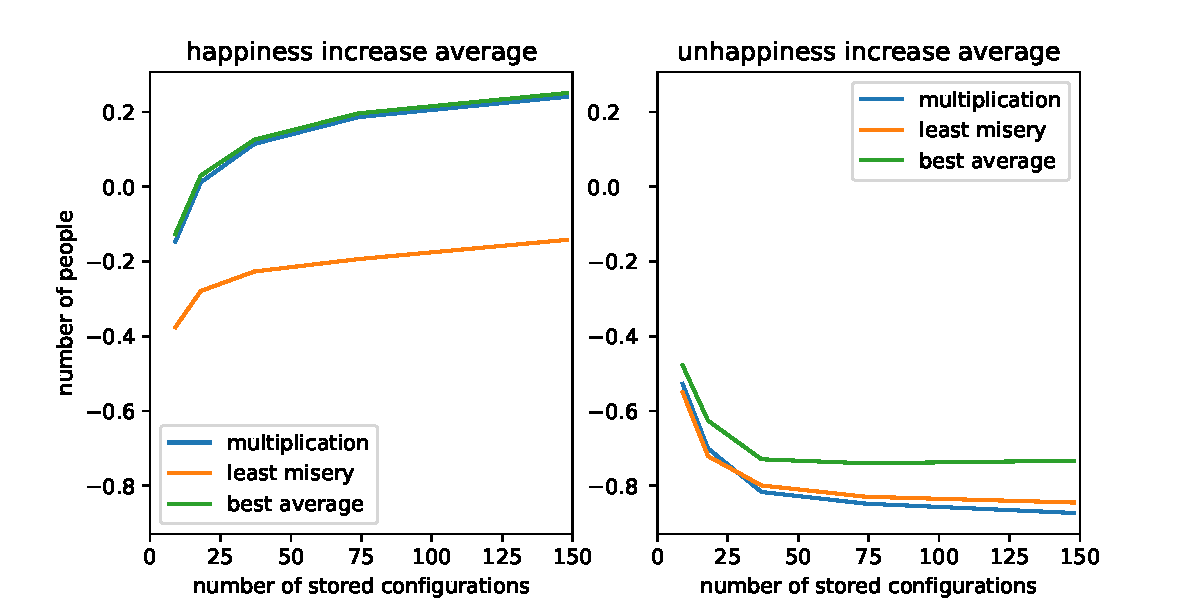
\includegraphics[width=1\textwidth]{./figures/60_evaluation/heterogeneous_happy_unhappy_increase_amount-1000_smd-15.pdf}
    \caption{The average satisfaction and dissatisfaction increase for \textbf{heterogeneous} groups consisting of four members with $smd=15\%$.}
    \label{fig:Evaluation:HeterogenousGroupIncrease}
\end{figure}

\begin{figure}
    \centering
    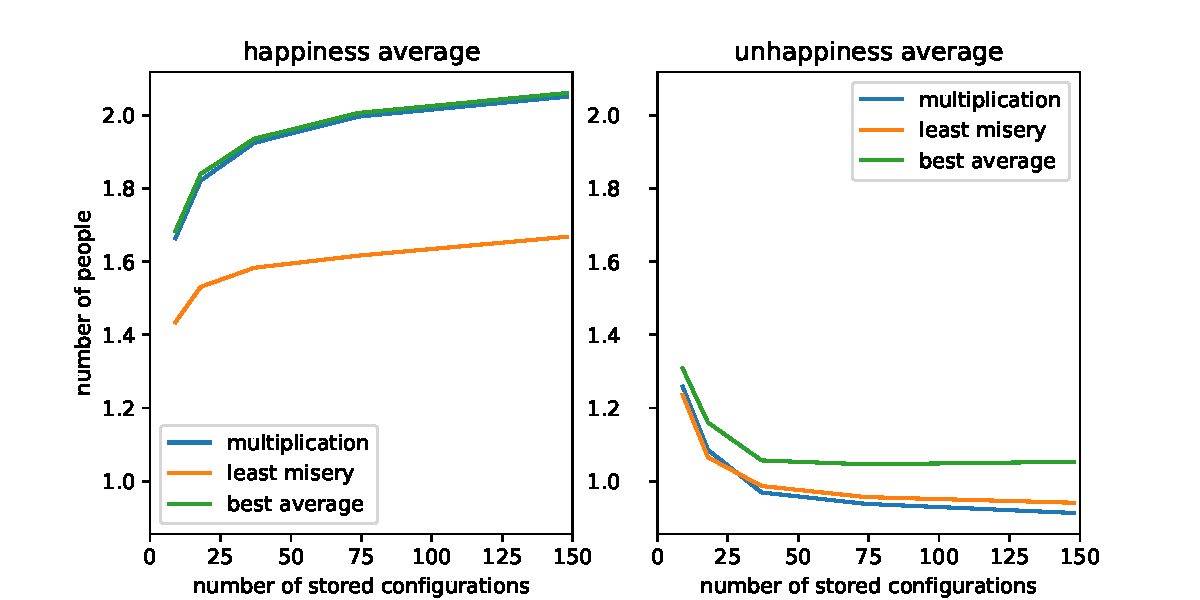
\includegraphics[width=1\textwidth]{./figures/60_evaluation/heterogeneous_happy_unhappy_total_group_amount-1000_smd-15.pdf}
    \caption{The average satisfaction and dissatisfaction for \textbf{heterogeneous} groups consisting of four members with $smd=15\%$.}
    \label{fig:Evaluation:HeterogenousGroupTotal}
\end{figure}

\begin{figure}
    \centering
    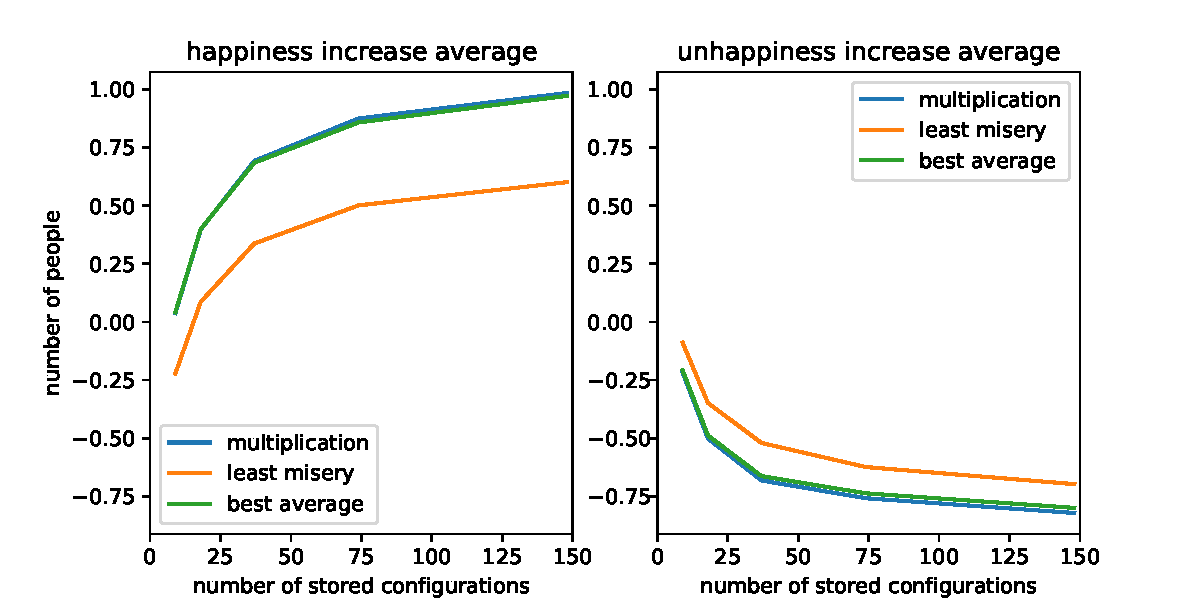
\includegraphics[width=1\textwidth]{./figures/60_evaluation/random_happy_unhappy_increase_amount-1000_smd-15.pdf}
    \caption{The average satisfaction and dissatisfaction increase for a \textbf{random} groups consisting of four members with $smd=15\%$.}
    \label{fig:Evaluation:RandomGroupIncrease}
\end{figure}

\begin{figure}
    \centering
    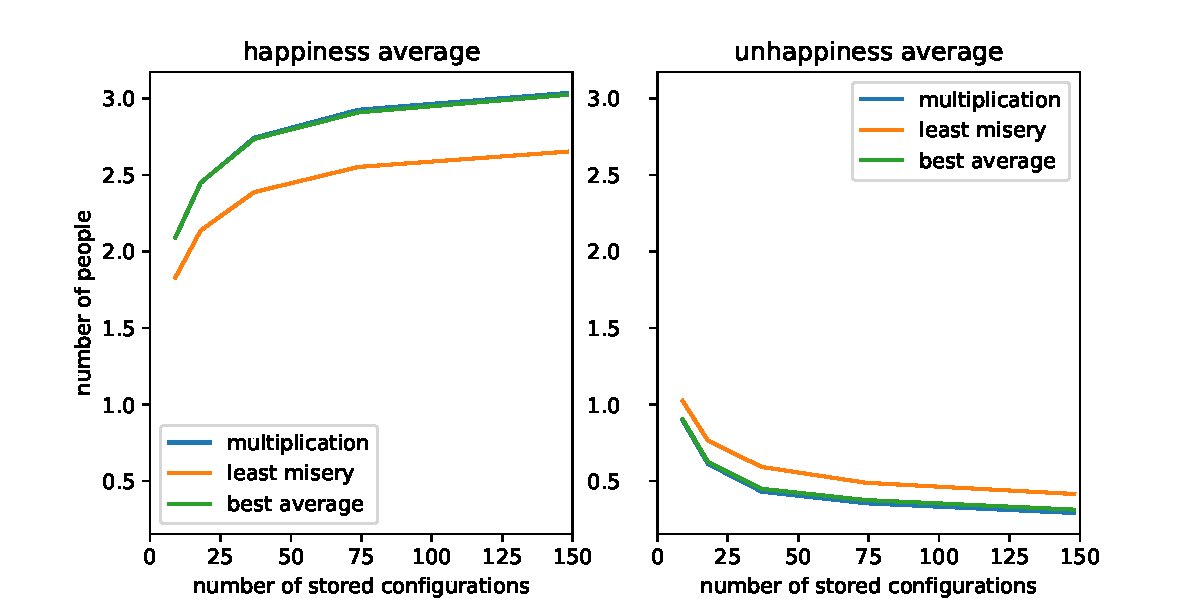
\includegraphics[width=1\textwidth]{./figures/60_evaluation/random_happy_unhappy_total_group_amount-1000_smd-15.pdf}
    \caption{The average satisfaction and dissatisfaction for \textbf{random} groups consisting of four members with $smd=15\%$.}
    \label{fig:Evaluation:RandomGroupTotal}
\end{figure}
